\structure{ПРАКТИЧЕСКАЯ ЧАСТЬ}

Параметры записи: частота дискретизации 11,025 кГц, разрядность 16 бит, режим
«моно», формат wav. Произносилась фраза: «Железцов Никита Владимирович,
двадцать шестое марта две тысячи двадцать пятого года. А, Э, И, О, У, Ы ». При
анализе речевого сигнала использовано программное обеспечение: Praat, Sound
Edit, WaveView.

\subsection*{Характеристики микрофона}

За последние несколько лет наряду с аналоговыми микрофонами все большее
применение находят цифровые микрофоны. Получение высококачественных
аудиозаписей в различной акустической обстановке обеспечивают цифровые
микрофоны, например Logitech USB Desktop Microphone (рис. \ref{fig:fig02}). По
данным компании разработчика, в микрофоне используется технология подавления
шумов, позволяющая отфильтровывать фоновые шумы, в частности сигналы «фона»
сети питания 50 Гц.

\begin{figure}
    \centering
    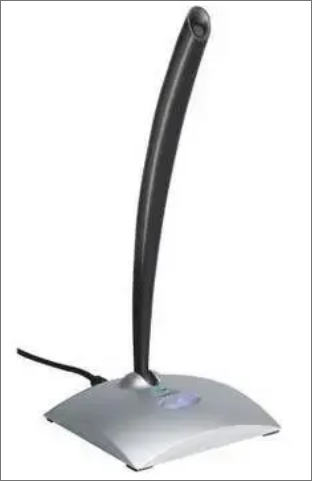
\includegraphics[scale=0.6]{inc/fig_02.png}
    \caption{ Внешний вид микрофона Logitech USB Desktop Microphone }
    \label{fig:fig02}
\end{figure}

Технические характеристики микрофона Logitech USB Desktop Microphone:

\begin{itemize}
    \item Разъем, тип А -USB
    \item Частотный диапазон, кГц - 100–16 000
    \item Чувствительность, дБ - 67
    \item Поддержка ОС - Windows 98 и старше, МаcOS 9.0.4 и старше
    \item Масса, кг - 0,392
\end{itemize}

\subsection*{Программа для анализа речи Praat}

Записанный материал был загружен в программу Praat. Перед проведением анализа
было выполнено конфигурирование приложения следующим образом. Характеристики
отображения Фурье-спектрограммы (англ. Spectrogram settings) представлены в
таблице 1.  Настройки показа формант (англ. Formants settings) - в таблице 2.
Параметры отображения траектории основного тона в координатах частота-время
(англ. Pitch settings) - в таблице 3.

\begin{table}[H]
\centering
\label{tab:tab01}
\caption{Настройки отображения Фурье-спектрограммы (Spectrogram settings)}
\begin{tabular}{|l|l|}
\hline
Параметр      & Значение        \\
\hline
View range    & 0--5000~Hz      \\
Window length & 0.005~s         \\
Dynamic range & 70.0~dB         \\
\hline
\end{tabular}
\end{table}

\begin{table}[H]
\centering
\label{tab:tab02}
\caption{Настройки показа формант (Formants settings)}
\begin{tabular}{|l|l|}
\hline
Параметр           & Значение      \\
\hline
Formant ceiling    & 5500~Hz       \\
Number of formants & 2             \\
Window length      & 0.04~s        \\
Dynamic range      & 24.0~dB       \\
Dot size           & 2.0~mm        \\
\hline
\end{tabular}
\end{table}

\begin{table}[H]
\centering
\label{tab:tab03}
\caption{Параметры отображения траектории основного тона (Pitch settings)}
\begin{tabular}{|l|l|}
\hline
Параметр     & Значение              \\
\hline
Pitch range  & 100--400.0~Hz         \\
Unit         & Hertz (логарифмический) \\
\hline
\end{tabular}
\end{table}

На рисунке \ref{fig:fig03} приведена Фурье-спектрограмма всей произнесённой
фразы, отмечена траектория основного тона в координатах
частота-время. Желтым цветом на рисунке \ref{fig:fig03} обозначена
интенсивность (intensity), синим цветом обозначена высота тона звука (pitch),
красным цветом обозначены форманты (formants).

\begin{figure}
    \centering
    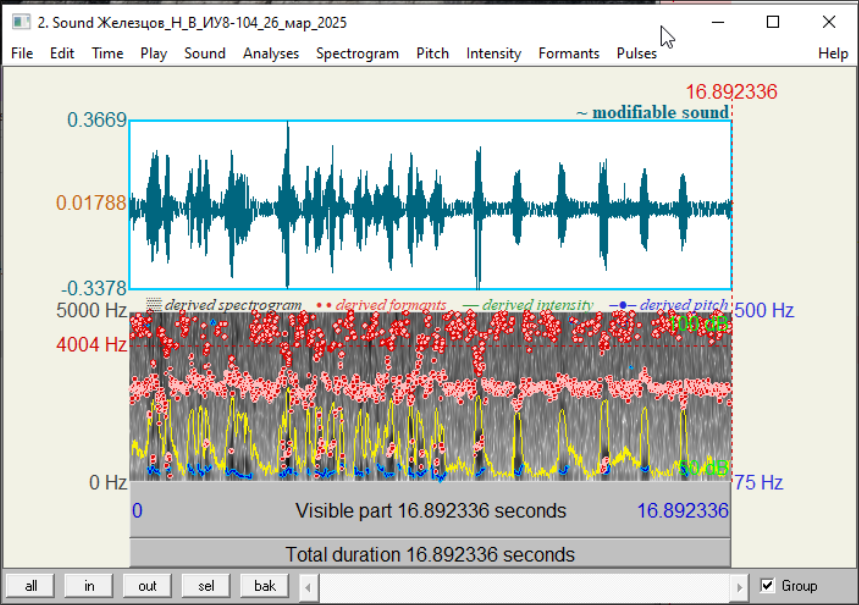
\includegraphics[scale=0.4]{inc/fig_03.png}
    \caption{
        Спектрограмма фразы «Железцов Никита Владимирович, двадцать шестое
        марта две тысячи двадцать пятого года. А, Э, И, О, У, Ы»
    }
    \label{fig:fig03}
\end{figure}

\subsection*{Звуковой редактор Sound Edit}

На рисунке \ref{fig:fig04} показана тестовая запись, а на рисунке
\ref{fig:fig05} показана Фурье-спектрограмма для тестовой записи, полученная с
использованием Sound Edit. На рисунке \ref{fig:fig06} – Вейвлет-сонограмма. На
рисунке \ref{fig:fig07} приведена Вейвлет-сонограмма для выделенных гласных
звуков «А, Э, И, О, У, Ы». Для отдельно выделенного звука «А» приведена
Фурье-спектрограмма и Вейвлет-сонограмма на рисунке \ref{fig:fig08}. Также
проанализирован спектр звука «А» с параметрами БПФ 512 и окном Блэкмана –
рисунок \ref{fig:fig09}.

\begin{figure}
    \centering
    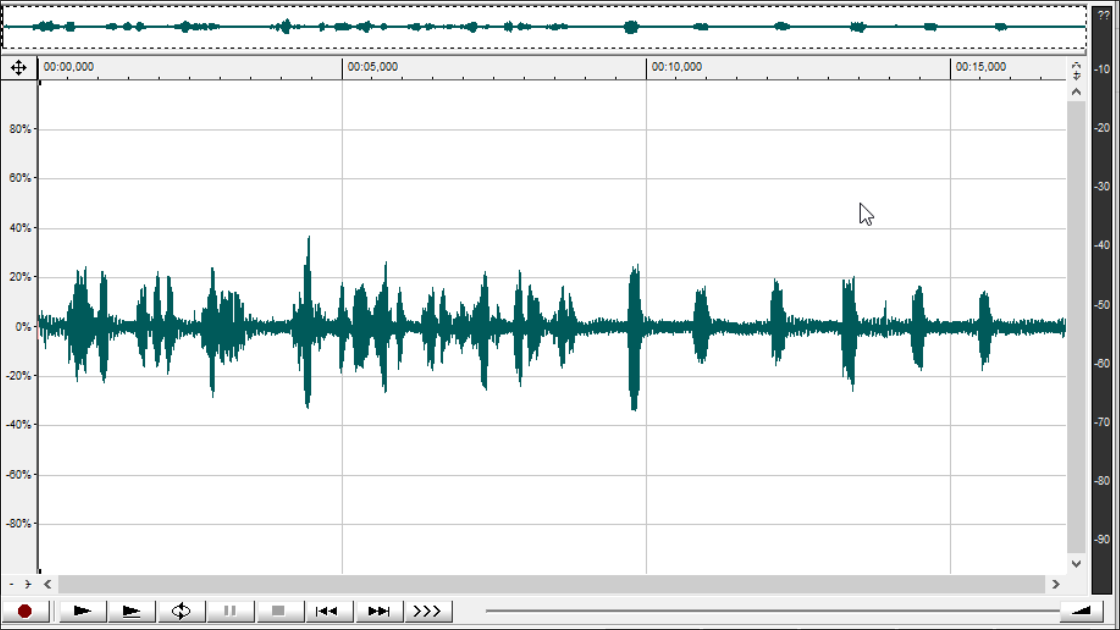
\includegraphics[scale=0.4]{inc/fig_04.png}
    \caption{Амплитуда тестовой записи в SoundEdit}
    \label{fig:fig04}
\end{figure}

\begin{figure}
    \centering
    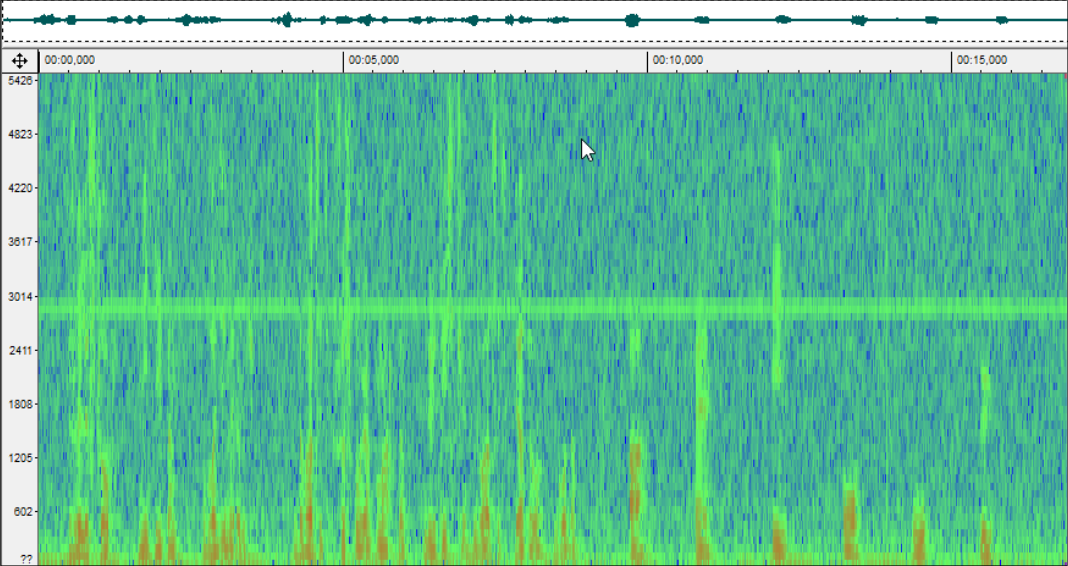
\includegraphics[scale=0.4]{inc/fig_05.png}
    \caption{Фурье-сонограмма тестовой записи в SoundEdit}
    \label{fig:fig05}
\end{figure}

\begin{figure}
    \centering
    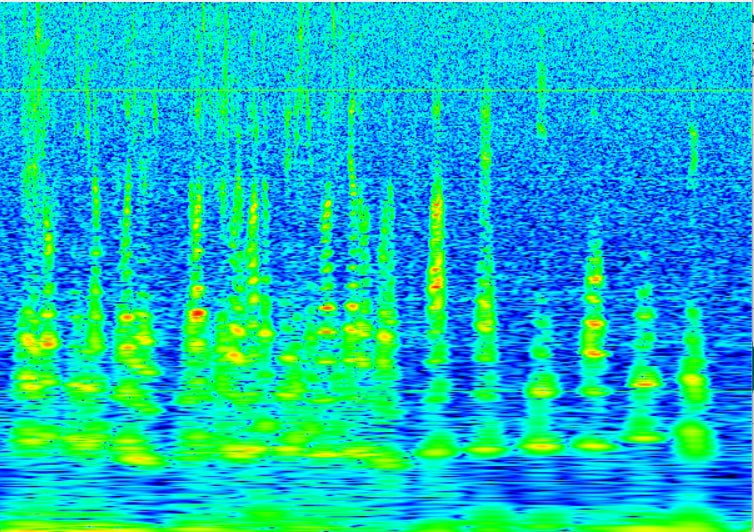
\includegraphics[scale=0.7]{inc/fig_06.jpg}
    \caption{Вейвлет-сонограмма тестовой записи в SoundEdit}
    \label{fig:fig06}
\end{figure}

\begin{figure}
    \centering
    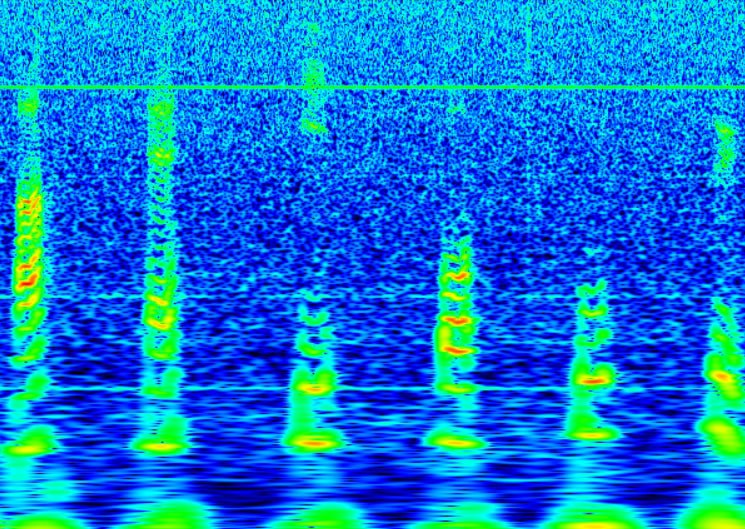
\includegraphics[scale=0.7]{inc/fig_07.jpg}
    \caption{Вейвлет-сонограмма гласных звуков «А, Э, И, О, У, Ы»}
    \label{fig:fig07}
\end{figure}

\begin{figure}
    \centering
    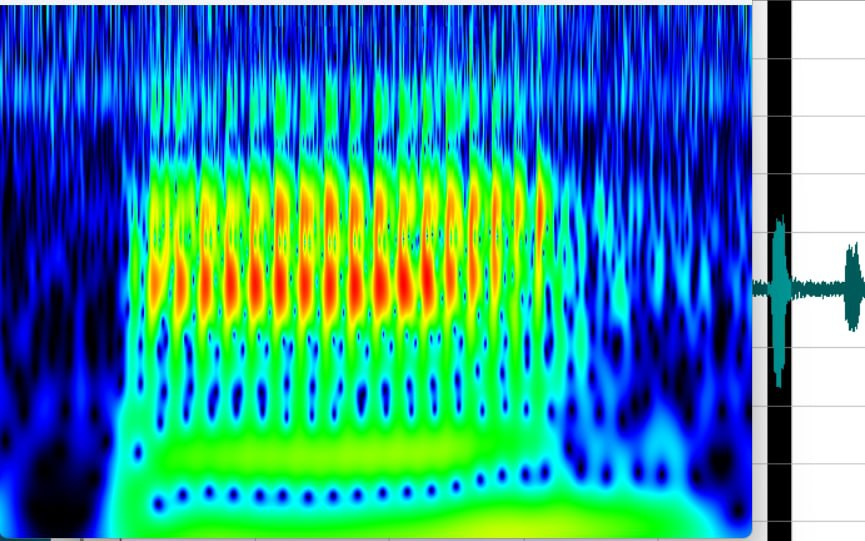
\includegraphics[scale=0.7]{inc/fig_08.jpg}
    \caption{Вейвлет-сонограмма гласного звука «А»}
    \label{fig:fig08}
\end{figure}

\begin{figure}
    \centering
    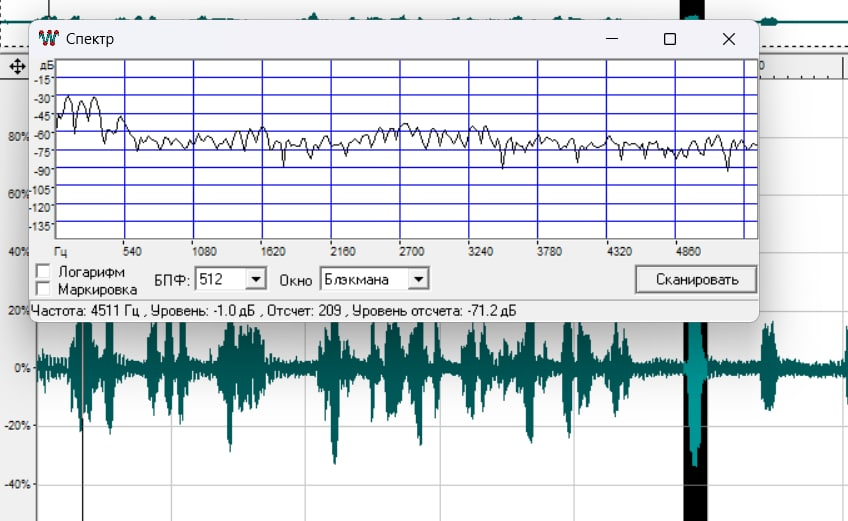
\includegraphics[scale=0.7]{inc/fig_09.jpg}
    \caption{Спектр гласного звука «А». БПФ 512, окно Блэкмана}
    \label{fig:fig09}
\end{figure}

\subsection*{Программа WaveView}

Необходимо отметить преимущество WaveView, которое заключается в возможности
выполнять полноценный вейвлет-анализ с последующим созданием
Вейвлет-сонограммы.

Так как человеческий голос является нестационарным сигналом, он не может быть
эффективным образом обработан средствами Фурье-анализа, использующего
разложение в сумму периодических функций. Ключевым свойством, которым обладает
Вейвлет-сонограмма и не обладает Фурье- спектрограмма, является локализация
особенностей сигнала, в том числе, низкочастотных.

В рамках анализа тестовой записи для звука «А» в программе WaveView построена
Вейвлет-сонограмма и частотное сечение. Определены частоты наиболее
энергетически сильных гармоник: первая гармоника соответствует частоте 127 Гц,
вторая – частоте 207 Гц. Результат показан на рисунке \ref{fig:fig10}.
При помощи возможностей WaveView по отображению временной позиции курсора было
определено время начала звука и время окончания, таким образом длительность
звука «А» составила 0,255 с.

\begin{figure}
    \centering
    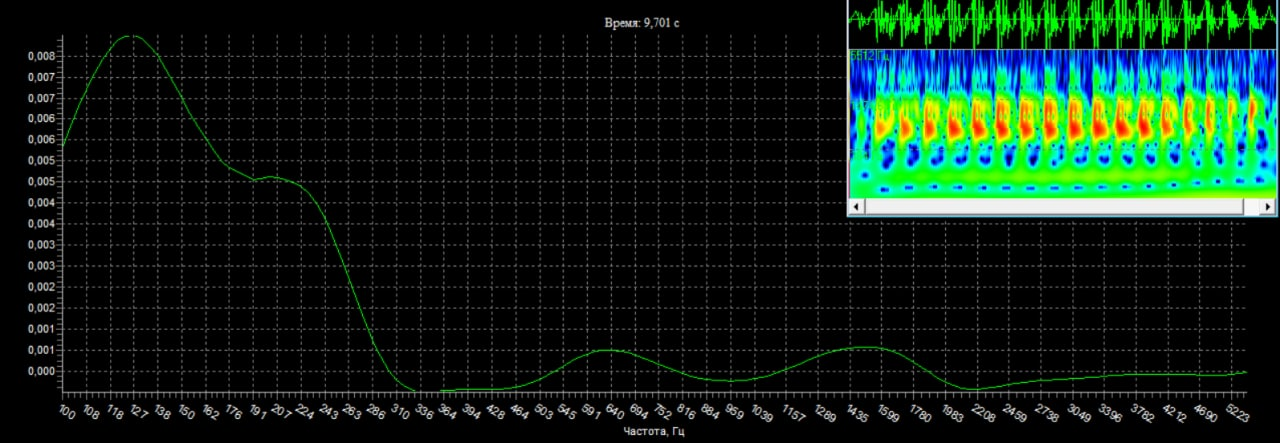
\includegraphics[scale=0.5]{inc/fig_10.jpg}
    \caption{
        Вейвлет-сонограмма гласного звука «А», сверху рисунка спектральное
        сечение выделенного участка сигнала 9,701 сек. Частота 1-й гармоники 127
        Гц, частота 2-й гармоники 207 Гц.
    }
    \label{fig:fig10}
\end{figure}

Аналогично для анализа согласных звуков был выбран звук был проанализирован
звук «В» в слове «двадцать», для него первая гармоника соответствует 88 Гц,
вторая – 170 Гц. Результат показан на рисунке \ref{fig:fig11}. Длительность
произнесения звука «В» на тестовой записи составляет 0,065 с.

\begin{figure}
    \centering
    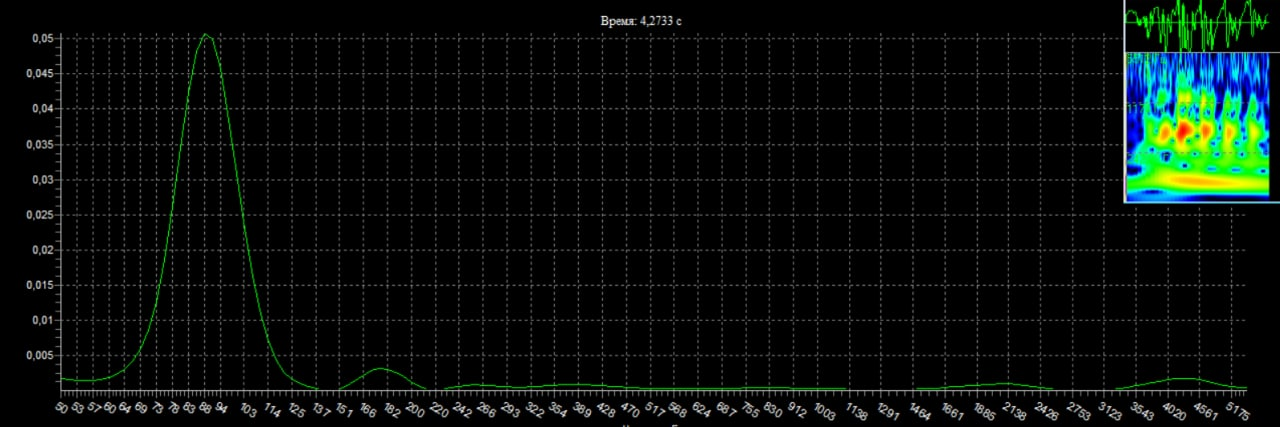
\includegraphics[scale=0.5]{inc/fig_11.jpg}
    \caption{
        Вейвлет-сонограмма согласного звука «В», сверху рисунка спектральное
        сечение выделенного участка сигнала 4,2733 сек. Частота 1-й гармоники
        88 Гц, частота 2-й гармоники 170 Гц.
    }
    \label{fig:fig11}
\end{figure}

Был проанализирован звук «Г» в слове «года», результат представлен на рисунке
\ref{fig:fig12}. Длительность произнесения звука на тестовой записи
составляет 0,102 с. Частота 1-й гармоники 114 Гц, частота 2-й гармоники 230 Гц.
Результат на рис. \ref{fig:fig12}.

\begin{figure}
    \centering
    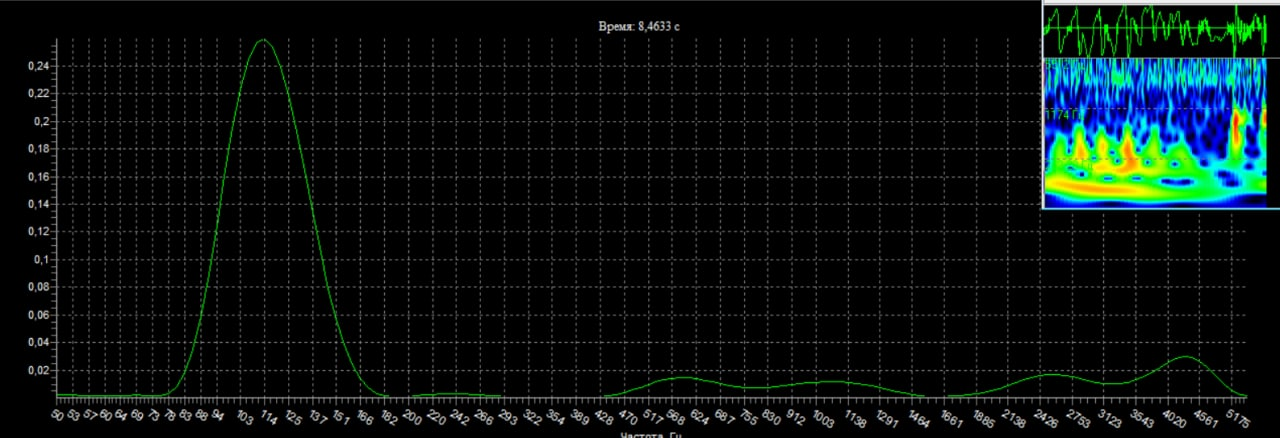
\includegraphics[scale=0.5]{inc/fig_12.jpg}
    \caption{
        Вейвлет-сонограмма согласного звука «Г», сверху рисунка спектральное
        сечение выделенного участка сигнала 8,4633 сек. Частота 1-й гармоники
        114 Гц, частота 2-й гармоники 230 Гц.
    }
    \label{fig:fig12}
\end{figure}
